
\documentclass{article}
\usepackage{tikz}
\usetikzlibrary{patterns}
\usepackage{graphicx} 
\usepackage{subfigure}
\usepackage{mathpazo}
\usepackage{pgfplots}
\newcommand*{\num}{pi}

\graphicspath{ {C:/Users/Jacki/Pictures/} }
\begin{document}

\begin{figure}
\center
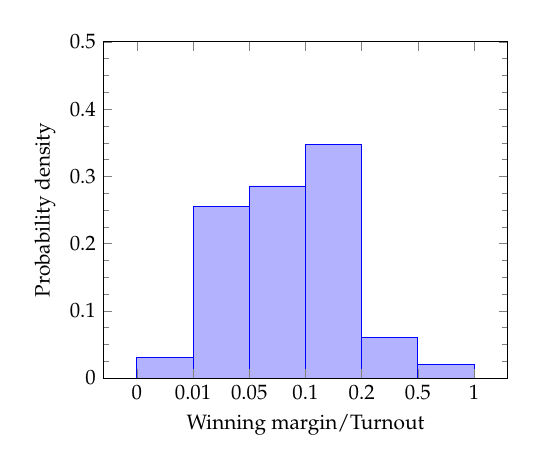
\begin{tikzpicture}[scale=0.75]
\begin{axis}[
    ylabel = Probability density,
    xlabel = Winning margin/Turnout,
    ymin=0, ymax=0.5,
    minor y tick num = 3,
    area style,
	xtick={0,2,4,6,8,10,12,14,16},
	xticklabels={$0$,$0$,$0.01$,$0.05$,$0.1$,$0.2$,$0.5$,$1$},
    ]
\addplot+[ybar interval,mark=no] plot coordinates { (2, 0.0306) (4, 0.255) (6, 0.2857) (8, 0.3469) (10, 0.061) (12,0.02) (14,0)};
\end{axis}
\end{tikzpicture}
\caption{1992-1999}

\center
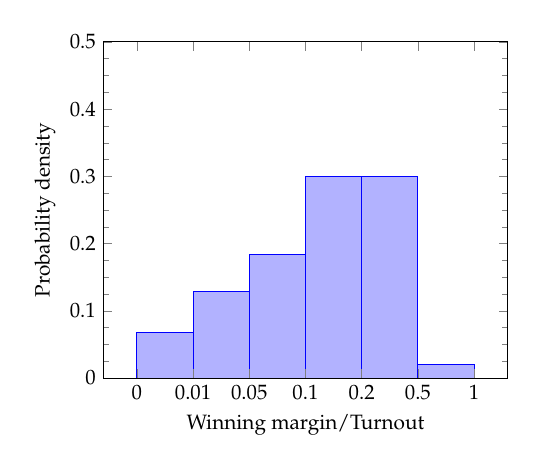
\begin{tikzpicture}[scale=0.75]
\begin{axis}[
    ylabel = Probability density,
    xlabel = Winning margin/Turnout,
    ymin=0, ymax=0.5,
    minor y tick num = 3,
    area style,
	xtick={0,2,4,6,8,10,12,14,16},
	xticklabels={$0$,$0$,$0.01$,$0.05$,$0.1$,$0.2$,$0.5$,$1$},
    ]
\addplot+[ybar interval,mark=no] plot coordinates { (2, 0.068) (4,0.1292) (6,0.1836) (8,0.2993) (10,0.2993) (12,0.0204) (14,0)};
\end{axis}
\end{tikzpicture}
\caption{2000-2009}

\center
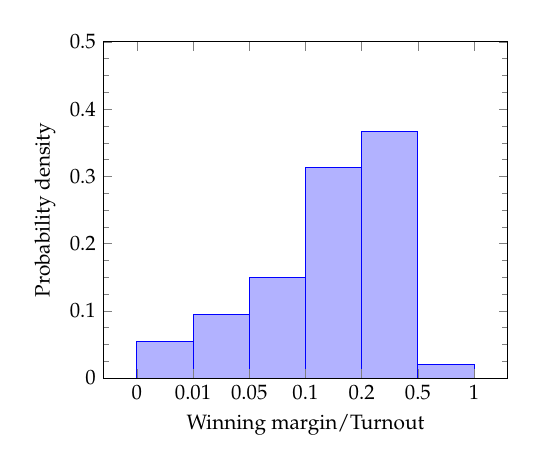
\begin{tikzpicture}[scale=0.75]
\begin{axis}[
    ylabel = Probability density,
    xlabel = Winning margin/Turnout,
    ymin=0, ymax=0.5,
    minor y tick num = 3,
    area style,
    xtick={0,2,4,6,8,10,12,14,16},
    xticklabels={$0$,$0$,$0.01$,$0.05$,$0.1$,$0.2$,$0.5$,$1$},
    ]
\addplot+[ybar interval,mark=no] plot coordinates { (2, 0.0544) (4, 0.09523) (6, 0.1496) (8, 0.31292) (10, 0.3673) (12,0.0204) (14,0)};
\end{axis}
\end{tikzpicture}
\caption{2010-2020}
\end{figure}

\end{document}